\documentclass[12pt]{extarticle}
\usepackage[left = 2cm, right = 2cm, top = 2cm, bottom = 2cm]{geometry}
\usepackage{graphicx}
\usepackage{amsmath}
\usepackage{amssymb}
\usepackage{hyperref}
\usepackage{listings}
\usepackage{multirow}
\usepackage{caption}
\usepackage{subcaption}
\usepackage{float}
\usepackage{placeins}

\begin{document}

\begin{flushleft}
\begin{LARGE}
\textbf{23.6}
\end{LARGE}  
\end{flushleft}

\vfill
\begin{center}
\begin{Huge}Accretion Discs\end{Huge}
\end{center}
\vfill

\pagebreak

\begin{center}
\textbf{Question 1}
\end{center}

Starting with the mass conservation equation, 

$$R\frac{\partial \Sigma}{\partial t} =-\frac{\partial}{\partial R}(R\Sigma V_R)$$

$$R\frac{\partial \Sigma}{\partial t} =-\frac{\partial}{\partial R}\left[\frac{1}{(R^2 \Omega)'} R\Sigma V_R(R^2 \Omega)'\right]$$

$$R\frac{\partial \Sigma}{\partial t}=-\frac{\partial}{\partial R}\left[\frac{1}{(R^2 \Omega)'}\left(R^2\Omega \left( R\frac{\partial \Sigma}{\partial t}+\frac{\partial}{\partial R}(R\Sigma V_R)\right)+R\Sigma V_R(R^2 \Omega)'\right)\right]$$

$$R\frac{\partial \Sigma}{\partial t}=-\frac{\partial}{\partial R}\left[\frac{1}{(R^2 \Omega)'}\left( R\frac{\partial (\Sigma R^2\Omega)}{\partial t}+\frac{\partial}{\partial R}(R\Sigma V_R R^2 \Omega)\right)\right]$$

$$R\frac{\partial \Sigma}{\partial t}=-\frac{\partial}{\partial R}\left[\frac{1}{2\pi (R^2 \Omega)'}\frac{\partial \Gamma}{\partial R} \right]$$


Where we have made use of conservation of mass again in the third line and conservation of angular momentum in the final line. We continue by applying the relations for the viscous torque and the angular velocity.

$$\frac{\partial \Sigma}{\partial t}=-\frac{1}{R}\frac{\partial}{\partial R}\left[\frac{1}{2\pi (R^2 (GM)^{1/2}R^{-3/2})'}\frac{\partial }{\partial R}(2\pi R \nu \Sigma R^2 ((GM)^{1/2}R^{-3/2})') \right]$$

$$\frac{\partial \Sigma}{\partial t}=-\frac{1}{R}\frac{\partial}{\partial R}\left[\frac{1}{(R^{1/2})'}\frac{\partial }{\partial R}\left(R \nu \Sigma R^2 \left(-\frac{3}{2}R^{-5/2}\right)\right) \right]$$

$$\frac{\partial \Sigma}{\partial t}=\frac{1}{R}\frac{\partial}{\partial R}\left[\frac{2}{R^{-1/2}}\frac{\partial }{\partial R}\left(\nu \Sigma \left(\frac{3}{2}R^{1/2}\right)\right) \right]$$

$$\frac{\partial \Sigma}{\partial t}=\frac{1}{R}\frac{\partial}{\partial R}\left[R^{1/2}\frac{\partial }{\partial R}(3\nu \Sigma R^{1/2}) \right]$$

This equation governs the evolution of the surface density of a Keplerian accretion disc.\\

\begin{center}
\textbf{Question 2}
\end{center}

We use both conservation equations to find a relation for the radial velocity.
$$R\frac{\partial(\Sigma R^2\Omega)}{\partial t}+\frac{\partial}{\partial R}(R\Sigma V_R R^2 \Omega) = \frac{\partial}{\partial R}(\nu \Sigma R^3 \Omega ')$$

$$R^2 \Omega \left(R\frac{\partial \Sigma}{\partial t}+\frac{\partial}{\partial R}(R\Sigma V_R)\right)+R\Sigma V_R\frac{\partial}{\partial R}(R^2 \Omega)  = \frac{\partial}{\partial R}(\nu \Sigma R^3 \Omega ')$$

$$R\Sigma V_R\frac{\partial}{\partial R}(R^2 (GMR^{-3})^{1/2})  = \frac{\partial}{\partial R}\left(\nu \Sigma R^3 ((GMR^{-3})^{1/2})'\right)$$

$$V_R = -\frac{3}{\Sigma R^{1/2}}\frac{\partial}{\partial R}(\nu \Sigma R^{1/2})$$

We substitute for the mass accretion rate $\dot{m}$. It follows directly from mass conservation that it is constant in a steady state.
$$ \frac{\dot{m}}{2\pi R\Sigma} = \frac{3}{\Sigma R^{1/2}}\frac{\partial}{\partial R}(\nu \Sigma R^{1/2})$$

$$\nu \Sigma R^{1/2} = \frac{\dot{m}}{3\pi}(R^{1/2}+A)$$

where $A$ is constant. We apply the inner boundary condition $\Sigma = 0$ at $R = R_{\mathrm{in}}$ to obtain
$$\nu \Sigma = \frac{\dot{m}}{3\pi}\left(1-\sqrt{\frac{R_{in}}{R}}\right)$$

The plot of this solution is shown in figure 1. We make the problem dimensionless by setting $r = R/R_0$, $\tau = t/t_0$, $\sigma (r,\tau) = \Sigma/\Sigma_0$ and $\eta (r,\tau) = \nu/\nu_0$ in the governing equation.
$$\frac{d\tau}{dt}\frac{\partial (\sigma \Sigma_0)}{\partial \tau}=\frac{1}{rR_0}\frac{dr}{dR}\frac{\partial}{\partial r}\left[(rR_0)^{1/2}\frac{dr}{dR}\frac{\partial }{\partial r}(3\eta\nu_0 \sigma \Sigma_0 (rR_0)^{1/2}) \right]$$

$$\frac{R_0^2}{\nu_0 t_0}\frac{\partial \sigma}{\partial \tau}=\frac{1}{r}\frac{\partial}{\partial r}\left[r^{1/2}\frac{\partial }{\partial r}(3\eta\sigma r^{1/2}) \right]$$

For the equation to remain the same we must have $t_0 = R_0^2/\nu_0$.\\

\begin{center}
\textbf{Question 3}
\end{center}

We make the substitution $X = r^{1/2}$. The derivative transforms as

$$\frac{\partial}{\partial r} = \frac{dX}{dr}\frac{\partial }{\partial X} = \frac{1}{2r^{1/2}}\frac{\partial }{\partial X} = \frac{1}{2X}\frac{\partial }{\partial X} $$

and the equation becomes

$$\frac{\partial \sigma}{\partial \tau}=\frac{1}{X^2}\frac{1}{2X}\frac{\partial}{\partial X}\left[X\frac{1}{2X}\frac{\partial }{\partial X}(3\eta \sigma X) \right]$$

$$\frac{\partial}{\partial \tau} (4\sigma X^3)=\frac{\partial^2}{\partial X^2}  (3\eta \sigma X)$$

$$\frac{\partial f}{\partial \tau}=\frac{\partial^2 g}{\partial X^2} $$

where we have defined $f(X,\tau) = 4\sigma X^3$ and $g(X,\tau) = 3\eta \sigma X$.\\

We will use a first order forward difference in $\tau$ to estimate $f_{\tau}$ and a second order central difference in $X$ to estimate $g_{XX}$.

$$\frac{\partial f(X_i,\tau_n)}{\partial \tau}  \approx \frac{f(X_i,\tau_n + \Delta \tau) - f(X_i,\tau_n)}{\Delta \tau} = \frac{f_i^{n+1} - f_i^n}{\Delta \tau}$$

$$\frac{\partial^2 g(X_i,\tau_n)}{\partial X^2} \approx \frac{g_X(X_i+\frac{1}{2}\Delta X, \tau_n)-g_X(X_i-\frac{1}{2}\Delta X, \tau_n) }{\Delta X}$$
$$ \approx \frac{g(X_i+\Delta X, \tau_n)-g(X_i, \tau_n)-(g(X_i, \tau_n)-g(X_i-\Delta X, \tau_n))}{(\Delta X)^2} = \frac{g^n_{i+1}-2g^n_{i}+g^n_{i-1}}{(\Delta X)^2}$$

We combine these to obtain the difference equation.

$$f_i^{n+1} = f_i^n +\frac{\Delta \tau}{(\Delta X)^2}(g^n_{i+1}-2g^n_{i}+g^n_{i-1})$$\\

\begin{center}
\textbf{Question 4}
\end{center}

We create grids for $f$, $g$ and $\sigma$ and use the difference equation and boundary conditions to recursively find the solutions. For formal stability the timestep must satisfy 
$$\Delta\tau \leq \frac{1}{2}(\Delta X)^2\frac{f}{g} = \frac{1}{2} (\Delta X)^2\frac{4\sigma X^3}{3\eta \sigma X}\leq \frac{2}{3} (0.02)^2\,2^2 \approx 0.00107$$

where the second inequality comes from taking the maximum value of $X$. In the computation we find we need to use a smaller value of $\Delta \tau  = 5 \times 10^{-7}$. The surface density plots are shown in figures 2 and 3. The distribution becomes smoother and shallower over time as the mass spreads out. More mass drifts towards the inner boundary than the outer.  \\

\begin{center}
\textbf{Question 5}
\end{center}

The height and position of the peak in the surface density is shown in table 1. The position of the peak moves inwards as mass shifts towards the central object. The height of the peak decreases as the mass spreads out.\\

We derive an expression for the total angular momentum. Consider an annulus of matter lying between $R$ and $R+\Delta R$ with mass $\Delta M = 2\pi R\Delta R \Sigma$. It has moment of inertia $\Delta I = R^2\Delta M$ and angular momentum $\Delta L = \Omega \Delta I = 2\pi \sqrt{GMR^3}\Sigma \Delta R$. We integrate to obtain the total angular momentum.
$$L(t) = \int_{R_{in}}^{R_{out}}2\pi \sqrt{GMR^3}\,\Sigma(R,t)\, d R = C\int_{r_{in}}^{r_{out}} r^{3/2}\,\sigma(r,t) \, d r$$

where, using the normalisation condition $L(0) = 1$, we find $C\approx 8.897$. We use the built-in function trapz on Matlab to compute the integral at each time point. The evolution of the total angular momentum is shown in figure 4. The plot shows it decreasing over time as mass escapes through the boundaries, taking angular momentum with it. \\

The position of the peak angular momentum density is shown in figure 5, where a curve of best fit was applied to the data (using the built-in fit function). It initially decreases, presumably due to mass shifting inwards. After $\tau \approx 0.1$ the peak moves outwards as the angular momentum drifts outwards.\\

Overall we find that the surface density shifts towards the central object as mass moves inwards, whilst the angular momentum drifts outwards.\\

\begin{center}
\textbf{Question 6}
\end{center}

Making the same change of variables as before, we have  $V_r = R_0 v_r/t_0$ where $v_r = dr/d \tau$ is the radial velocity in dimensionless units. Applying them to the equation for $V_R$ and using the relation for $t_0$ we obtain

$$\frac{R_0}{t_0}v_r = -\frac{3}{\sigma \Sigma_0 (rR_0)^{1/2}}\frac{1}{ R_0}\frac{\partial }{\partial r}(\eta \nu_0 \sigma\Sigma_0 (rR_0)^{1/2}) $$

$$v_r = -\frac{3}{\sigma r^{1/2}}\frac{\partial }{\partial r}(\eta \sigma r^{1/2})$$

$$v_r = -\frac{3}{\sigma X}\frac{dX}{dr}\frac{\partial }{\partial X}(\eta \sigma X)$$

$$v_r = -\frac{1}{2\sigma X^2}\frac{\partial g}{\partial X}$$

We obtain a difference equation by using a forward difference for $g_X$

$$(v_r)_i^n = -\frac{1}{2\sigma_i^n (X_i)^2}\frac{g_{i+1}^n - g_i^n}{\Delta X}$$

The radial velocity at several timesteps is shown in figure 6. It is mostly positive for $r>1$, where the mass drifts outwards, and mostly negative for $r<1$, where it drifts inwards. Initially, it is greater in magnitude  for $r<1$, agreeing with the faster spread to the left we see in figure 3.\\

\begin{center}
\textbf{Question 7}
\end{center}

The particles' orbits are plotted in figure 7 for a range of initial radii. Linear interpolation was used in the program to determine the velocity at each point. A first order Euler procedure was used to numerically integrate the differential equation.\\

The maximum radii attained by the particles as well as the times taken to reach these are shown in figure 8. From these plots we can describe the trajectories according to initial radius.
\begin{itemize}
\item[-] $0.900<r_0< 0.974$. Paths of always decreasing radius. 
\item[-] $0.974< r_0< 0.984$. Paths of initially increasing and then decreasing radius.
\item[-] $0.984< r_0< 1.011$. Paths of always increasing radius which do not reach the outer boundary.
\item[-] $1.011<r_0<1.100$. Paths of increasing radius that reach the outer boundary. \\
\end{itemize}

For the particles that do reach a boundary, the times taken for them to do so are plotted in figure 9. Both follow smooth curves, with particles at the extremes taking less time, as expected.\\ \\ \\ \\

\begin{center}
\textbf{Question 8}
\end{center}

Using the plots in figure 9 we find that particles with initial radii $r_0 < 0.969$ have reached the inner boundary by $\tau = 0.512$. Integrating the initial distribution (using the built-in integral function) we find these particles make up a proportion of 0.235 of the initial mass. For the outer boundary we find the range is $r_0 > 1.08$ and the fraction is 0.042. These are particles that have escaped the accretion disc and so these proportions make up the lost mass.\\

Integrating the surface density at $\tau = 0.512$ we find the proportion of the original mass remaining is 0.413. Since mass is conserved, the total of these three proportions should equal 1. We however find $0.235+0.042+0.413 = 0.690$, a figure substantially lower than what is expected. This discrepancy can be attributed to an accumulation of numerical errors. 

\pagebreak 

\begin{center}
\textbf{Figures and Tables}
\end{center}

\begin{figure}[!htbp]
\centering
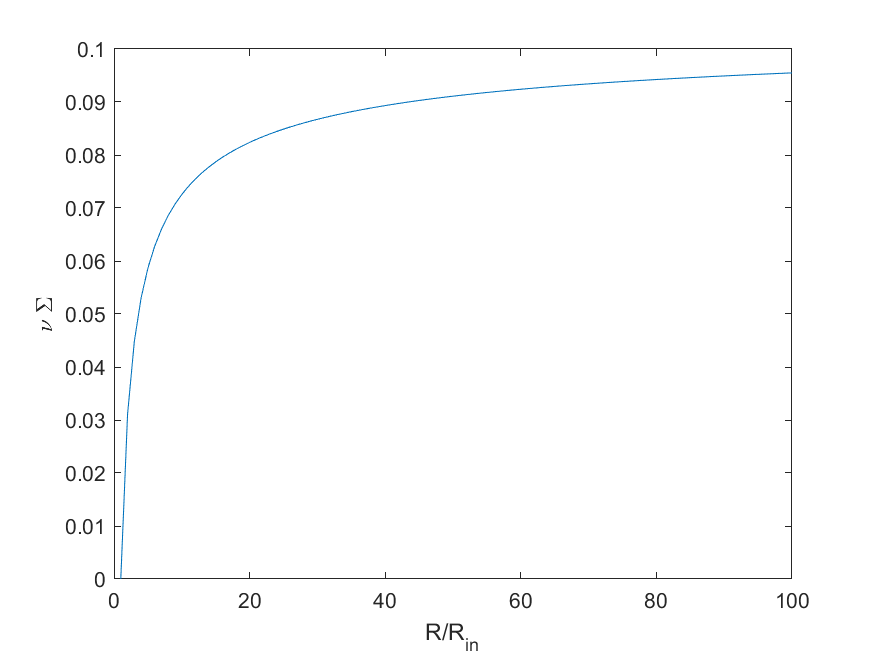
\includegraphics[scale=0.8]{Q2.png}
\caption{Plot of $\nu \Sigma$ in units of $\dot{m}$ against $R/R_{\mathrm{in}}$}
\label{figure:1}
\end{figure}

\begin{figure}[!htbp]
\centering
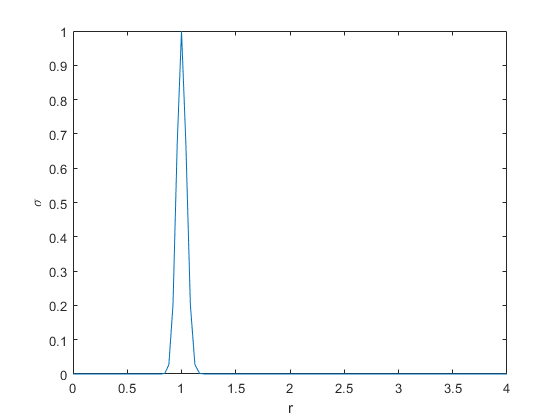
\includegraphics[scale=0.8]{Sigma1.png}
\caption{Plot of the initial surface density, $\sigma(r,0)$ against $r$}
\label{figure:2}
\end{figure}

\begin{figure}[!htbp]
\centering
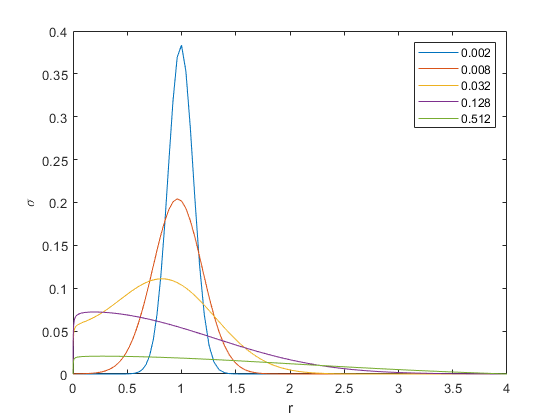
\includegraphics[scale=0.8]{Sigma2.png}
\caption{Plots of $\sigma$ against $r$ at several time points}
\label{figure:3}
\end{figure}

\begin{table}[!htbp]
\centering
\begin{tabular}{|c|cccccc|}
\hline
\multirow{1}{8em}{time, $\tau$} & 0 & 0.002 & 0.008 & 0.032 & 0.128 & 0.512 \\
\hline
\multirow{1}{8em}{Position of Peak} & 1.00 & 1.00 & 0.960 & 0.810 & 0.194 & 0.270\\
\hline
\multirow{1}{8em}{Height of Peak} & 1.00 & 0.383 & 0.204 & 0.111 & 0.0723 & 0.0208\\
\hline
\end{tabular}
\caption{Height and position of the peak in the surface density}
\label{Table:1}
\end{table}

\begin{figure}[!htbp]
\centering
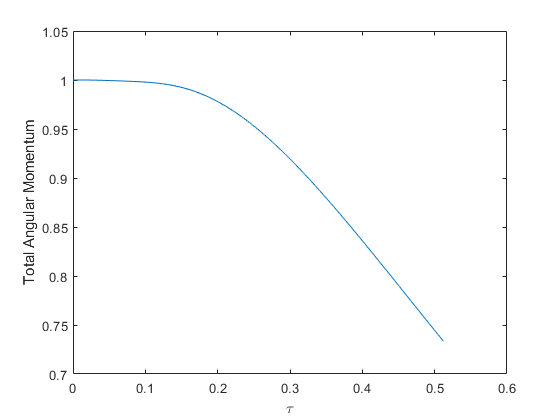
\includegraphics[scale=0.8]{TotalAngular.png}
\caption{Time evolution of the total angular momentum}
\label{figure:4}
\end{figure}

\begin{figure}[!htbp]
\centering
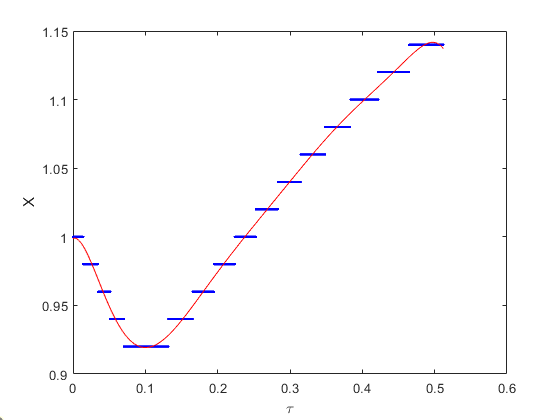
\includegraphics[scale=0.8]{PeakAngular.png}
\caption{Position of the peak angular momentum surface density ($R^2\Omega \Sigma$) against time}
\label{figure:5}
\end{figure}

\begin{figure}[!htbp]
\centering
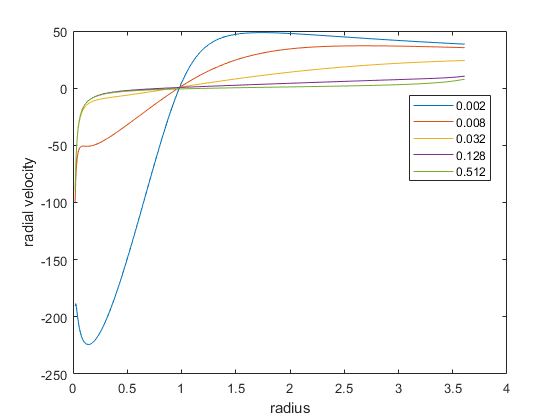
\includegraphics[scale=0.8]{RadialVelocity.png}
\caption{The radial velocity at several time points}
\label{figure:6}
\end{figure}

\begin{figure}[!htbp]
    \centering
    \begin{subfigure}[b]{0.47\textwidth}
        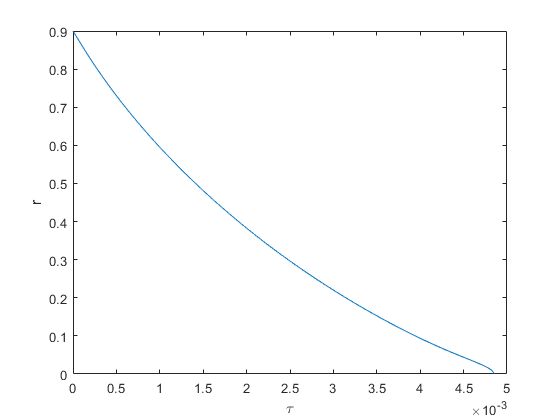
\includegraphics[width=\textwidth]{r0_0.9.png}
        \caption{$r_0 = 0.9$}
        \label{figure:7a}
    \end{subfigure}  
    \qquad
    \begin{subfigure}[b]{0.47\textwidth}
        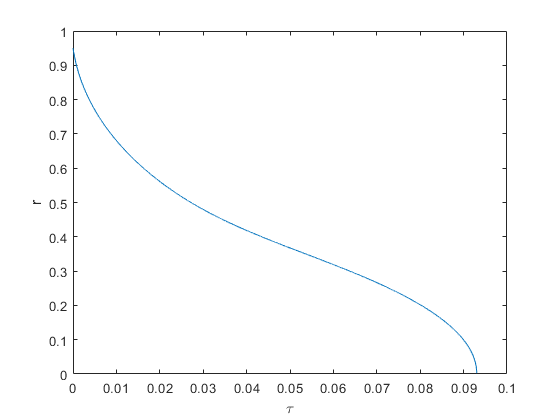
\includegraphics[width=\textwidth]{r0_0.95.png}
        \caption{$r_0 = 0.95$}
        \label{figure:7b}
    \end{subfigure} 
    \\ 
    \begin{subfigure}[b]{0.47\textwidth}
        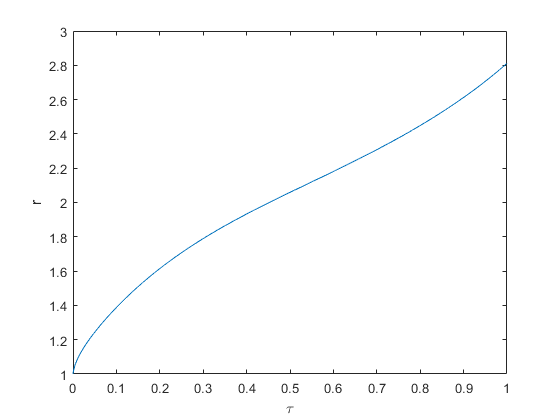
\includegraphics[width=\textwidth]{r0_1.0.png}
        \caption{$r_0 = 1.0$}
        \label{figure:7c}
    \end{subfigure} 
    \qquad
    \begin{subfigure}[b]{0.47\textwidth}
        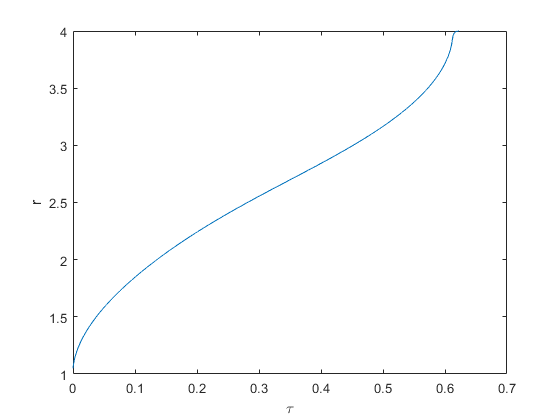
\includegraphics[width=\textwidth]{r0_1.05.png}
        \caption{$r_0 = 1.05$}
        \label{figure:7d}
    \end{subfigure}
      \\
    \begin{subfigure}[b]{0.47\textwidth}
        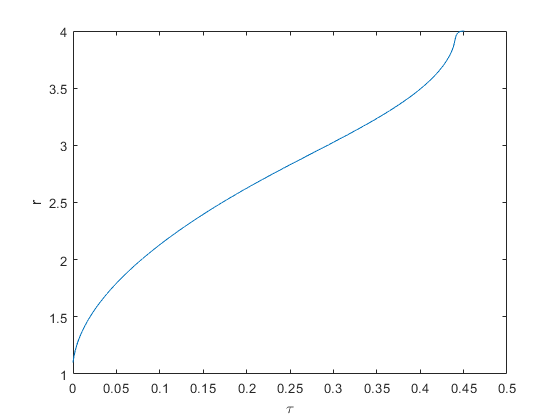
\includegraphics[width=\textwidth]{r0_1.1.png}
        \caption{$r_0 = 1.1$}
        \label{figure:7e}
    \end{subfigure}
    \caption{Evolution of particles' orbits}
    \label{figure 7}
\end{figure}

\begin{figure}[!htbp]
    \centering
    \begin{subfigure}[b]{0.47\textwidth}
        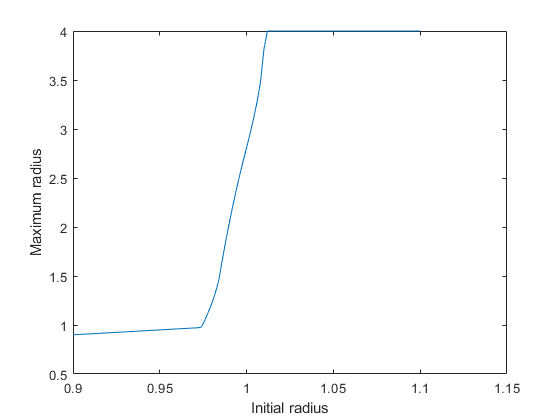
\includegraphics[width=\textwidth]{Distance_max.png}
        \caption{Maximum radius}
        \label{figure:8a}
    \end{subfigure}  
    \qquad
    \begin{subfigure}[b]{0.47\textwidth}
        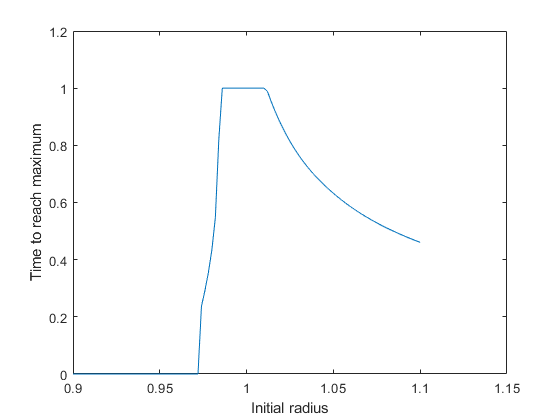
\includegraphics[width=\textwidth]{Time_max.png}
        \caption{Time taken to reach maximum}
        \label{figure:8b}
    \end{subfigure}
    \caption{Maximum radius attained and time taken to reach it}
    \label{figure 8}
\end{figure}

\begin{figure}[!htbp]
    \centering
    \begin{subfigure}[b]{0.47\textwidth}
        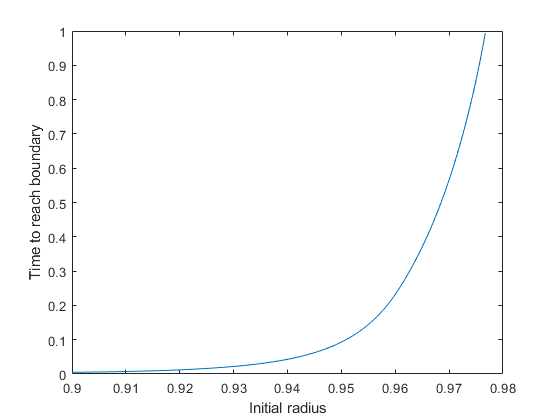
\includegraphics[width=\textwidth]{LowerBoundary.png}
        \caption{Inner boundary}
        \label{figure:9a}
    \end{subfigure}  
    \qquad
    \begin{subfigure}[b]{0.47\textwidth}
        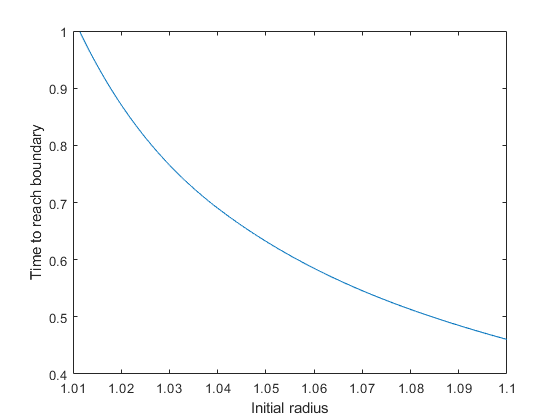
\includegraphics[width=\textwidth]{UpperBoundary.png}
        \caption{Outer boundary}
        \label{figure:9b}
    \end{subfigure}
    \caption{Time taken to reach either boundary}
    \label{figure 9}
\end{figure}

\pagebreak

\begin{center}
\textbf{Code Listings}
\end{center}

\begin{center}
Question 2
\end{center}
\lstinputlisting[language=Matlab]{Question2.m}

\begin{center}
Sigma
\end{center}
\lstinputlisting[language=Matlab]{Sigma.m}

\begin{center}
Question 4
\end{center}
\lstinputlisting[language=Matlab]{Question4.m}

\begin{center}
Question 5
\end{center}
\lstinputlisting[language=Matlab]{Question5.m}

\begin{center}
Radial velocity $v_r$
\end{center}
\lstinputlisting[language=Matlab]{V_R.m}

\begin{center}
Question 6
\end{center}
\lstinputlisting[language=Matlab]{Question6.m}

\begin{center}
Question 7
\end{center}
\lstinputlisting[language=Matlab]{Question7.m}

\begin{center}
Question 8
\end{center}
\lstinputlisting[language=Matlab]{Question8.m}

\end{document}
